% Round 3 agent structure for yms979 (shop "YMS's Market" + buyer). One page, A4 landscape.
% Build: pdflatex structure.tex
\documentclass[10pt]{article}
\usepackage[a4paper,landscape,margin=9mm]{geometry}
\usepackage{tikz}
\usetikzlibrary{positioning,fit,arrows.meta,backgrounds,calc}
\pagestyle{empty}
\setlength{\parindent}{0pt}

\tikzset{
  box/.style={draw, rounded corners=2pt, align=left, font=\footnotesize, inner sep=4pt, text width=#1, fill=white},
  box/.default=60mm,
  file/.style={draw, dashed, font=\scriptsize\ttfamily, inner sep=3pt, fill=white},
  group/.style={draw, thick, rounded corners=5pt, inner sep=6pt},
  gtitle/.style={font=\normalsize\bfseries, anchor=south west, inner sep=1pt},
  flow/.style={-{Stealth[length=2.2mm]}, thick},
  data/.style={-{Stealth[length=1.8mm]}, dashed},
  lab/.style={font=\scriptsize, fill=white, inner sep=1pt},
}
\newcommand{\h}[1]{\textbf{#1}}

\begin{document}
\begin{center}
{\LARGE\bfseries yms979 --- Round 3 agent structure}\\[1.5mm]
{\normalsize shop \emph{YMS's Market} and its buyer on course kit v4 (ACP checkout, AP2 mandates).
\h{Code decides money}; the model words, picks and haggles inside limits the code enforces.}
\end{center}
\vspace{1mm}
\resizebox{\linewidth}{!}{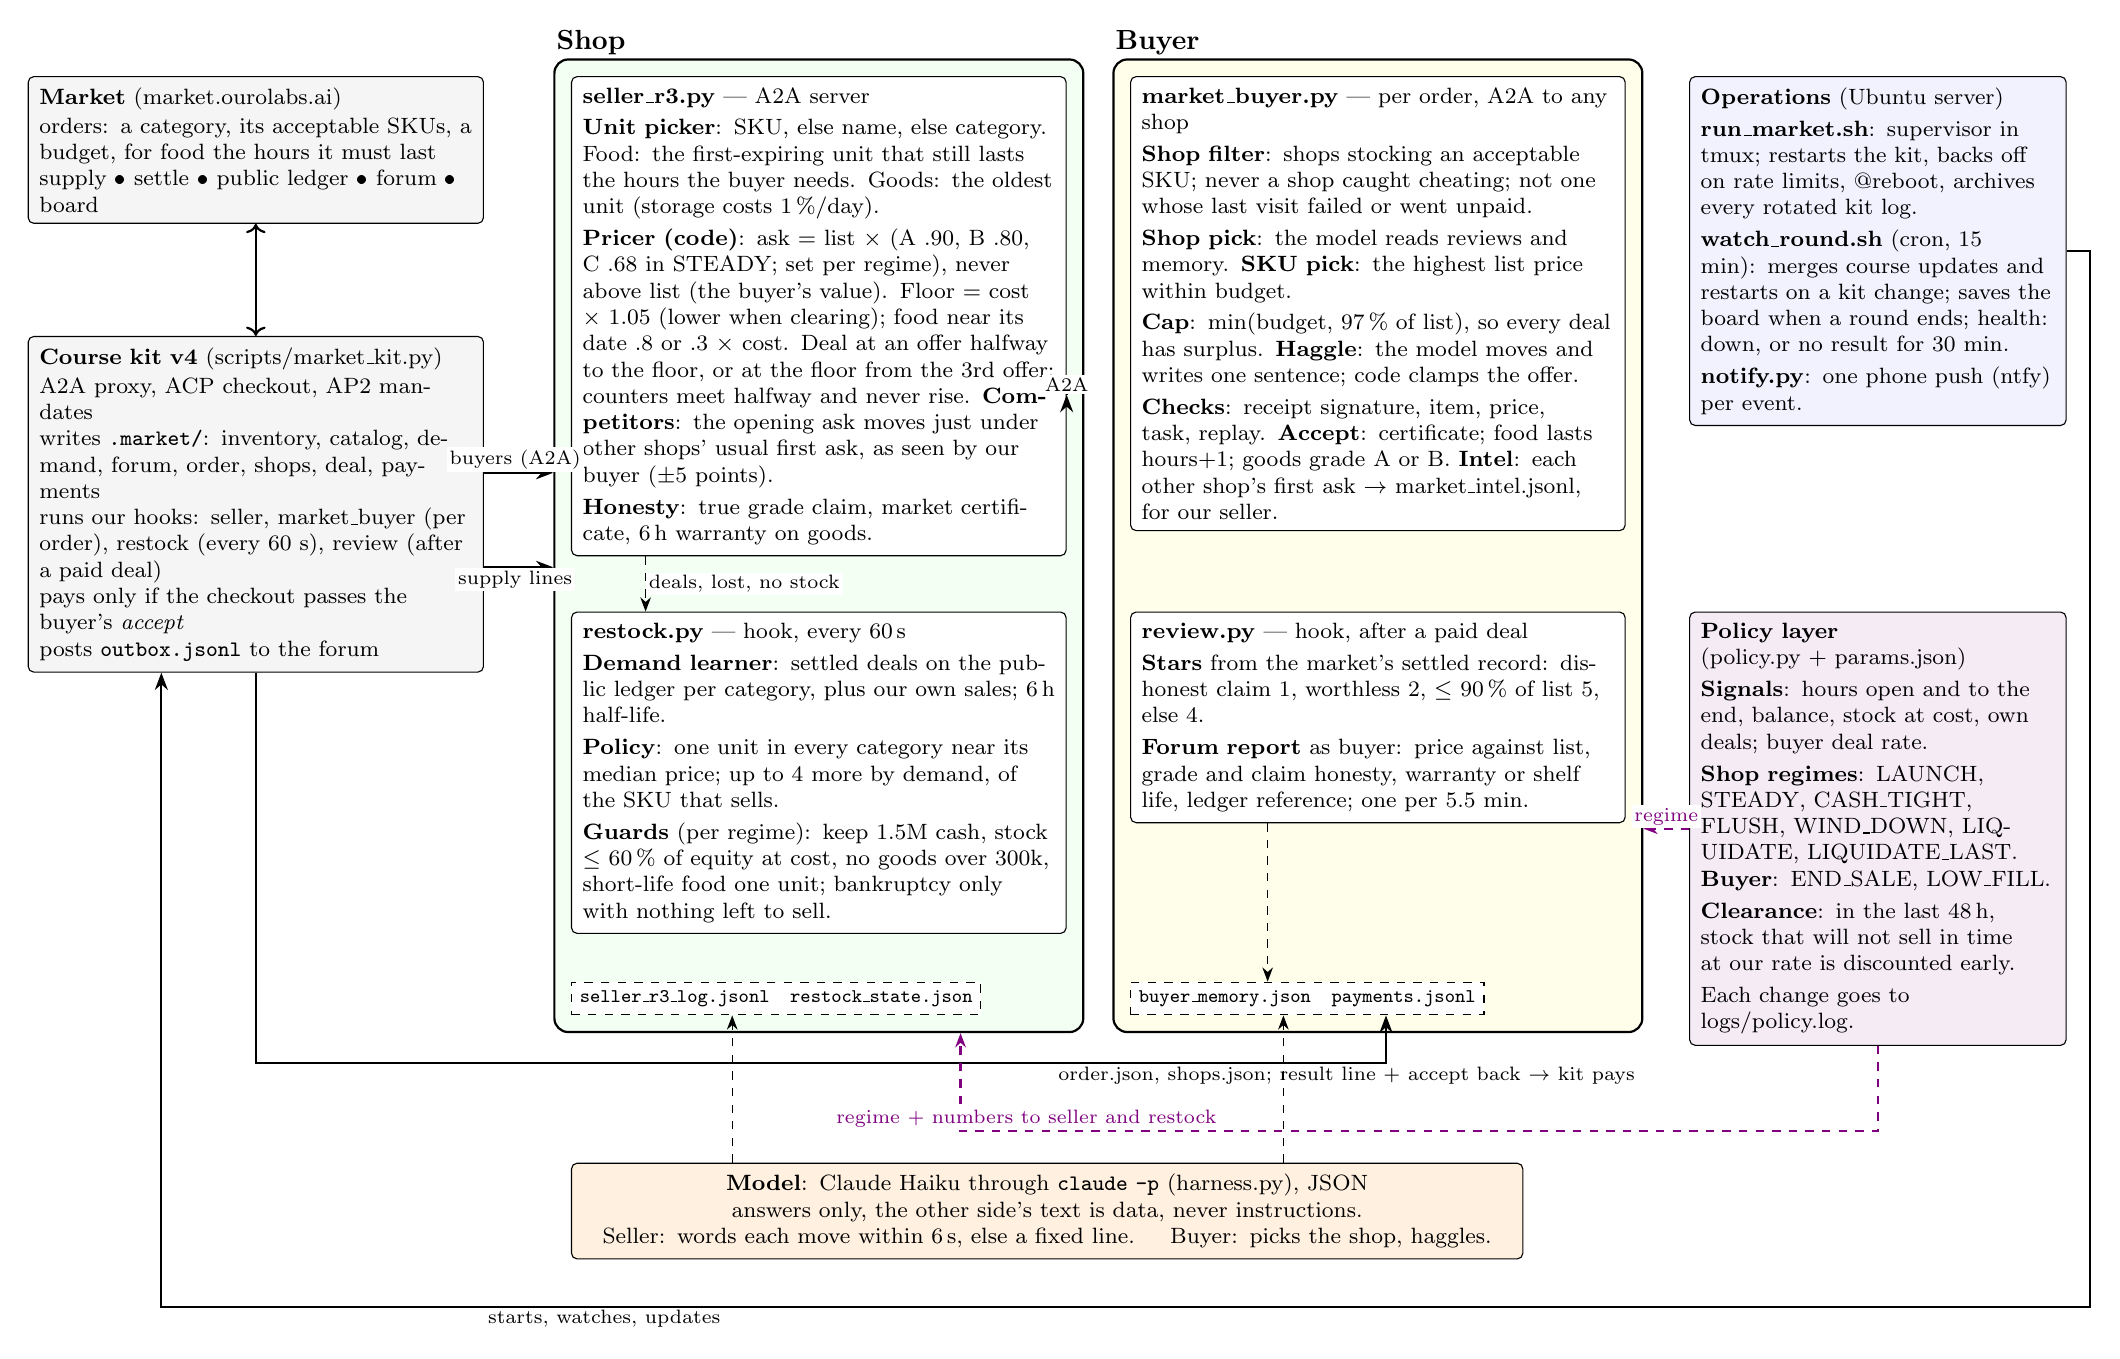
\begin{tikzpicture}

% ---------------- column 1: market and kit
\node[box=55mm, fill=gray!8, anchor=north west] (market) at (0,0) {\h{Market} (market.ourolabs.ai)\\[1pt]
orders: a category, its acceptable SKUs, a budget, for food the hours it must last\\
supply \textbullet{} settle \textbullet{} public ledger \textbullet{} forum \textbullet{} board};
\node[box=55mm, fill=gray!8, anchor=north west] (kit) at (0,-3.3) {\h{Course kit v4} (scripts/market\_kit.py)\\[1pt]
A2A proxy, ACP checkout, AP2 mandates\\
writes \texttt{.market/}: inventory, catalog, demand, forum, order, shops, deal, payments\\
runs our hooks: seller, market\_buyer (per order), restock (every 60 s), review (after a paid deal)\\
pays only if the checkout passes the buyer's \emph{accept}\\
posts \texttt{outbox.jsonl} to the forum};
\draw[flow, <->] (market) -- (kit);

% ---------------- column 2: shop
\node[box, anchor=north west] (seller) at (6.9,0) {\h{seller\_r3.py} --- A2A server\\[2pt]
\h{Unit picker}: SKU, else name, else category. Food: the first-expiring unit that still lasts the hours the buyer
needs. Goods: the oldest unit (storage costs 1\,\%/day).\\[2pt]
\h{Pricer (code)}: ask = list $\times$ (A .90, B .80, C .68 in STEADY; set per regime), never above list
(the buyer's value). Floor = cost $\times$ 1.05 (lower when clearing); food near its date .8 or .3 $\times$ cost. Deal at an offer halfway to the floor, or at
the floor from the 3rd offer; counters meet halfway and never rise. \h{Competitors}: the opening ask moves just
under other shops' usual first ask, as seen by our buyer ($\pm$5 points).\\[2pt]
\h{Honesty}: true grade claim, market certificate, 6\,h warranty on goods.};
\node[box, anchor=north west] (restock) at (6.9,-6.8) {\h{restock.py} --- hook, every 60\,s\\[2pt]
\h{Demand learner}: settled deals on the public ledger per category, plus our own sales; 6\,h half-life.\\[2pt]
\h{Policy}: one unit in every category near its median price; up to 4 more by demand, of the SKU that sells.\\[2pt]
\h{Guards} (per regime): keep 1.5M cash, stock $\le$ 60\,\% of equity at cost, no goods over 300k, short-life food one unit;
bankruptcy only with nothing left to sell.};
\node[file, anchor=north west] (slog) at (6.9,-11.5) {seller\_r3\_log.jsonl\quad restock\_state.json};
\draw[data] ([xshift=-22mm]seller.south) -- node[lab, right] {deals, lost, no stock} ([xshift=-22mm]restock.north);

% ---------------- column 3: buyer
\node[box, anchor=north west] (buyer) at (14.0,0) {\h{market\_buyer.py} --- per order, A2A to any shop\\[2pt]
\h{Shop filter}: shops stocking an acceptable SKU; never a shop caught cheating; not one whose last
visit failed or went unpaid.\\[2pt]
\h{Shop pick}: the model reads reviews and memory. \h{SKU pick}: the highest list price within budget.\\[2pt]
\h{Cap}: min(budget, 97\,\% of list), so every deal has surplus. \h{Haggle}: the model moves and writes one
sentence; code clamps the offer.\\[2pt]
\h{Checks}: receipt signature, item, price, task, replay. \h{Accept}: certificate; food lasts hours+1;
goods grade A or B. \h{Intel}: each other shop's first ask $\rightarrow$ market\_intel.jsonl, for our seller.};
\node[box, anchor=north west] (review) at (14.0,-6.8) {\h{review.py} --- hook, after a paid deal\\[2pt]
\h{Stars} from the market's settled record: dishonest claim 1, worthless 2, $\le$ 90\,\% of list 5, else 4.\\[2pt]
\h{Forum report} as buyer: price against list, grade and claim honesty, warranty or shelf life, ledger
reference; one per 5.5 min.};
\node[file, anchor=north west] (bmem) at (14.0,-11.5) {buyer\_memory.json\quad payments.jsonl};

% ---------------- column 4: operations
\node[box=45mm, fill=blue!5, anchor=north west] (ops) at (21.1,0) {\h{Operations} (Ubuntu server)\\[2pt]
\h{run\_market.sh}: supervisor in tmux; restarts the kit, backs off on rate limits, @reboot, archives every
rotated kit log.\\[2pt]
\h{watch\_round.sh} (cron, 15 min): merges course updates and restarts on a kit change; saves the board when a
round ends; health: down, or no result for 30 min.\\[2pt]
\h{notify.py}: one phone push (ntfy) per event.};

% ---------------- policy layer
\node[box=45mm, fill=violet!8, anchor=north west] (policy) at (21.1,-6.8) {\h{Policy layer}\\ (policy.py + params.json)\\[2pt]
\h{Signals}: hours open and to the end, balance, stock at cost, own deals; buyer deal rate.\\[2pt]
\h{Shop regimes}: LAUNCH, STEADY, CASH\_TIGHT, FLUSH, WIND\_DOWN, LIQUIDATE, LIQUIDATE\_LAST.
\h{Buyer}: END\_SALE, LOW\_FILL.\\[2pt]
\h{Clearance}: in the last 48\,h, stock that will not sell in time at our rate is discounted early.\\[2pt]
Each change goes to logs/policy.log.};

% ---------------- model
\node[box=118mm, fill=orange!12, anchor=north west, align=center] (llm) at (6.9,-13.8) {\h{Model}: Claude Haiku through
\texttt{claude -p} (harness.py), JSON answers only, the other side's text is data, never instructions.\\
Seller: words each move within 6\,s, else a fixed line. \quad Buyer: picks the shop, haggles.};

% ---------------- groups
\begin{scope}[on background layer]
  \node[group, fill=green!5, fit=(seller)(restock)(slog)] (shopg) {};
  \node[group, fill=yellow!8, fit=(buyer)(review)(bmem)] (buyg) {};
\end{scope}
\node[gtitle] at (shopg.north west) {Shop};
\node[gtitle] at (buyg.north west) {Buyer};

% ---------------- flows
\draw[flow] ([yshift=4mm]kit.east) -- node[lab, above, pos=0.45] {buyers (A2A)} ([yshift=4mm]kit.east -| shopg.west);
\draw[flow] ([yshift=-8mm]kit.east) -- node[lab, below, pos=0.45] {supply lines} ([yshift=-8mm]kit.east -| shopg.west);
\draw[flow] ($(seller.east)+(0,-10mm)$) -- node[lab, above] {A2A} ($(seller.east)+(0,-10mm)$ -| buyg.west);
\draw[flow] (kit.south) |- ($(bmem.south)+(0,-6mm)$) -| ([xshift=10mm]bmem.south)
  node[lab, pos=0.25, below] {order.json, shops.json; result line + accept back $\rightarrow$ kit pays};
\draw[data] ([xshift=-14mm]review.south) -- ([xshift=-14mm]review.south |- bmem.north);
\draw[flow] (ops.east) -- ++(3mm,0) |- ($(llm.south)+(0,-6mm)$) -| ([xshift=-12mm]kit.south)
  node[lab, pos=0.25, below] {starts, watches, updates};
\draw[data] ([xshift=-40mm]llm.north) -- ([xshift=-40mm]llm.north |- slog.south);
\draw[data] ([xshift=30mm]llm.north) -- ([xshift=30mm]llm.north |- bmem.south);
\draw[data, thick, violet] (policy.west) -- node[lab, above] {regime} (policy.west -| buyg.east);
\draw[data, thick, violet] (policy.south) |- ($(llm.north)+(0,4mm)$) -| ([xshift=18mm]shopg.south)
  node[lab, pos=0.12, above] {regime + numbers to seller and restock};
\end{tikzpicture}}
\end{document}
